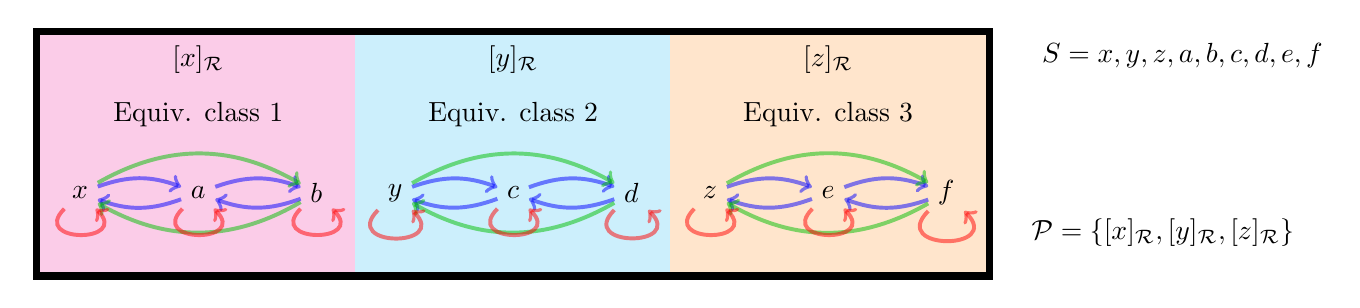
\begin{tikzpicture}
	\tikzset{
		main node/.style={circle, draw, fill=blue!20, minimum size=1cm, font=\sffamily},
		class node/.style={ellipse, draw, thick, red, minimum height=2.5cm, minimum width=4cm, align=center},
		path/.style={->, thick, shorten <=2pt, shorten >=2pt},
		reflexive/.style={->, line width=.5mm, loop, looseness=4, in=-45, out=225, red, opacity=.5},
		symmetric/.style={->, line width=.5mm, blue, bend left=20, opacity=.5},
		transitive/.style={->, line width=.5mm, green!75!black, bend left=30pt, opacity=.5},
		label distance=3mm
	}
	% Set S boundary
	\draw [thick, line width=2mm] (-6,-1) rectangle (6,2);
	\node at (8.5, 1.75) {$S=\set{x,y,z,a,b,c,d,e,f}$};
	
	% First equivalence class [x]R
	\filldraw[magenta!20] (-6,-1) rectangle (-2,2);
%	\draw[rounded corners, dashed, magenta, line width=.5mm] (-6,-1) rectangle (-2,2);
	\node at (-4, 1.7) {$[x]_\mathcal{R}$};
	\node at (-4, 1) {Equiv. class 1};
	\node (x) at (-5.5, 0) {$x$};
	\node (a) at (-4, 0) {$a$};
	\node (b) at (-2.5, 0) {$b$};
	
	% Second equivalence class [y]R
	\filldraw[cyan!20] (-2,-1) rectangle (2,2);
	\node at (0, 1.7) {$[y]_\mathcal{R}$};
	\node at (0, 1) {Equiv. class 2};
	\node (y) at (-1.5, 0) {$y$};
	\node (c) at (0, 0) {$c$};
	\node (d) at (1.5, 0) {$d$};
	
	% Third equivalence class [z]R
	\filldraw[orange!20] (2,-1) rectangle (6,2);
	\node at (4, 1.7) {$[z]_\mathcal{R}$};
	\node at (4, 1) {Equiv. class 3};
	\node (z) at (2.5, 0) {$z$};
	\node (e) at (4, 0) {$e$};
	\node (f) at (5.5, 0) {$f$};
	
	% Label for partition
	\node at (8.25, -.5) {$\mathcal{P} = \{ [x]_\mathcal{R}, [y]_\mathcal{R}, [z]_\mathcal{R} \}$};
	
	\foreach \x/\y in {x/a, a/b, y/c, c/d, z/e, e/f} {
		\draw[symmetric] (\x) to (\y);
		\draw[symmetric] (\y) to (\x);
	}
	
	\foreach \x/\y in {x/b, y/d, z/f} {
		\draw[transitive] (\x) to (\y);
		\draw[transitive] (\y) to (\x);
	}
	
	\foreach \x in {x,y,z,a,b,c,d,e,f} {
		\draw[reflexive] (\x) to (\x);
	}
	
\end{tikzpicture}